\chapter{Treiber}
\label{chap:Treiber}

\section{Architektur des Multi-Wan Bonding fähigen Windows Treibers}
\subsection{Design}
\subsubsection{Anforderungen}
Unser Multi-Wan Bonding Treiber ist dafür verantwortlich Pakete aus Windows zu dem Server zu senden. Dabei müssen 3 Probleme gelöst werden:
\newline
\begin{itemize}
    \item Sammeln von IP Paketen aus Windows
    \item Verteilen von IP Paketen an Programme
    \item Kommunikation zwischen Treiber und Server
\end{itemize}
\ \\
Außerdem müssen gewisse Standards von Performance, Stabilität und Ressourcenintensität gehalten werden. Dabei haben wir versucht folgende Metriken einzuhalten:
\newline
\begin{itemize}
    \item Maximale prozentuale CPU Auslastung von 5 \%, bei einer 100 Mbit/s Übertragungsrate auf einem (Prozessor von Tests einsetzten)
    \item Maximaler Speicherverbrauch von 300 Mega Byte bei Verwendung von 2 übertragenen Netzwerkadaptern über eine Dauer von 30 Minuten.
    \item Wenn es zum Absturz des Treibers kommen sollte, darf das Betriebssystem nicht mit abstürzen.
    \item Der Treiber sollte weiter funktionieren, auch wenn während des Betriebs ein Netzwerkadapter ausfällt.
\end{itemize}
\ \\
Zur Bedienungsfreundlichkeit wird ein Command Line Interface (CLI)  zur Verfügung gestellt mit welcher folgende Operationen ermöglicht werden:
\newline
\begin{itemize}
    \item Konfigurieren des Treibers über JSON, Key-Value Dateien oder über die Konsole
    \item Starten und Stoppen der Kommunikation des Treibers mit dem Server
    \item Stoppen und Starten des Treibers
    \item Ausgabe von derzeitigen Einstellungen
\end{itemize}
\ \\
Die CLI soll über eine lokale TCP Verbindung mit dem Treiber kommunizieren damit sichergestellt werden kann das andere Komponenten leicht eingebunden werden können.


\subsection{Sammeln von IP Paketen in Windows}
Damit Pakete an den Server versendet werden können, müssen wir dafür sorgen, dass Pakete die von verschiedenen Programmen in Windows verschickt werden durch unseren Treiber leiten. Um Pakete entgegennehmen zu können muss ein virtueller Netzwerkadapter erstellt werden. Dazu verwenden wir den Netzwerktreiber Wintun\footnote[1]{\url{https://www.wintun.net/}, 2021-01-16 23:19 MEZ}. Dieser kann performant Pakete empfangen und versenden.
\newline
\newline
Wintun kann jetzt zwar Pakete empfangen. Windows weiß aber noch nicht das es Pakete in den virtuellen Netzwerkadapter umleiten muss. Dafür muss eine statische IP Route im Windows internen IP Routing Table\footnote[2]{\url{https://docs.microsoft.com/en-us/windows-server/administration/windows-commands/route_ws2008}, 2021-01-16 23:30 MEZ} eingetragen werden.
\newline
\newline
Nach diesen 2 Schritten werden von Programmen gesendete Pakete, von Windows mithilfe  der Informationen im IP Routing Table, an den Wintun Adapter gesendet und dort durch unseren Treiber verarbeitet. (Für Details siehe Abbildung 7.1)
\begin{figure}[H]
    \centering
    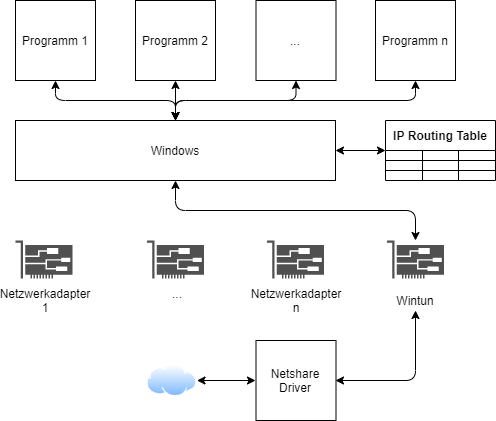
\includegraphics[width=0.8\textwidth]{diagramm_sammel_von_ip_paketen.png}
    \caption[Sammeln von IP Paketen]{Sammeln von IP Paketen} 
\end{figure}
\newpage


\subsection{Kommunikation zwischen Mulit-Wan Bonding Treiber und Mulit-Wan Bonding Server}
Der Treiber kann jetzt Pakete von Windows erhalten und muss diese an den Server schicken. Hierzu war die erste Entscheidung, die wir fällen mussten, auf welche Art wir die Pakete an den Server schicken. Dafür hatten wir zwei Möglichkeiten. Wir verwenden Wintun zum Senden und Empfangen der Pakete vom Server oder wir erstellen einen Socket und lassen über diesen die Kommunikation mit dem Server laufen.
\newline
\newline
Wenn, wir Wintun verwenden haben wir den Vorteil das wir keine weitere externe Bibliothek benutzen müssen und eine höhere Performance haben, weil wir Pakete von OSI Schicht 3 versenden und uns dadurch eine Schicht beim Senden sparen.
\newline
\newline
Der Grund warum wir uns aber dazu entschieden haben Sockets zu nutzen ist der Programmieraufwand. Wir haben zwar bei Wintun eine Performance Steigerung jedoch würde es auch bedeuten, dass wir uns mit dem Aufbau der einzelnen IP Pakete beschäftigen müssen. Was alleine akzeptabel wäre, wenn wir uns nicht auch noch um die Firewalls kümmern müssten. Dadurch das Firewalls weiter oben im OSI Modell angelegt sind als unser TUN Gerät\footnote[1]{\url{https://petri.com/csc_routers_switches_and_firewalls}, 2021-02-01 18:03 MEZ}, müssen wir beim Empfangen von Paketen sicherstellen, das die Firewall diese nicht wegwirft. Das heißt, wir müssen Windows mitteilen, dass wir einen gewissen Port benutzen und Pakete von einer gewissen IP-Adresse erwarten. Aus diesen beiden Gründen und durch unseren bestehenden Zeitdruck haben wir uns dazu entschieden eine Socket Bibliothek zu verwenden.
\newline
\newline
Für die Socket Bibliothek haben wir uns dann für die Windows Sockets 2 API entschieden, weil diese von Microsoft für das Performante verwenden von Sockets unter Windows entwickelt wurde. Außerdem haben wir den Vorteil das wir die Bibliothek nicht selber verwalten müssen, weil diese automatisch von Windows aktualisiert wird.


\subsection{Pakete aus dem Mulit-Wan Bonding Treiber auf andere Programme des Betriebssystems aufteilen}
Nachdem wir jetzt Pakete einsammeln können, diese dann an den Server schicken und empfangen können, müssen wir uns nur mehr sicherstellen, dass wir die Pakete aus unserem Treiber wieder an die Programme verteilen können, zu denen sie gehören. 
\newline
\newline
Hierfür machen wir uns wieder Wintun zu nutzen, indem wir die Pakete, die wir bekommen haben, nehmen und einfach über unser Wintun Gerät senden. Windows erkennt dann, dass das Paket an sich selbst gerichtet ist und verarbeitet es als wäre es von einem normalen Netzwerk Adapter gekommen. Durch diese Art der Aufteilung lagern wir den meisten Programmieraufwand an Windows aus und können auch für eine hohe Performance garantieren.
\newpage
Fügt man nun alle 3 Überlegungen zusammen, kommt man auf Folgendes. (Siehe Abbildung 7.2)
\begin{figure}[H]
    \centering
    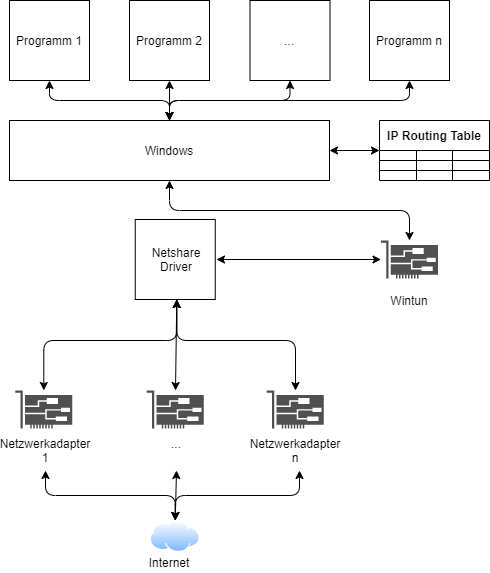
\includegraphics[width=0.8\textwidth]{kommunikation_mit_internet.png}
    \caption[Vollständige Mulit-Wan Bonding Treiber Architektur]{Vollständige Mulit-Wan Bonding Treiber Architektur} 
\end{figure}
\newpage
\section{Implementierung}
\subsection{IP Pakete Life Cylce}
\subsubsection{Erstellen des Eintrags in die IP Routing Tabelle}
Um IP Pakete umleiten zu können müssen wir Einträge in den IP Routing Table von Windows einfügen. Wie die Codebase des Multi-Wan Bonding Treibers noch nicht ausgereift genug war, haben wir diese Einträge über die Konsole mithilfe des \textbf{route} Befehls eingefügt. Um Pakete in unser Virtual Network Interface Card (VNIC) umleiten zu können müssen wir eine \textbf{default route} erstellen. Als Gateway stellen wir dann die IP-Adresse der VNIC des Mulit-Wan Bonding Servers und als Schnittstelle wählen wir die IP-Adresse der VNIC von unserem Mulit-Wan Bonding Treiber. Als Metrik haben wir die kleinste Metrik gewählt, die über den route Befehl erstellt werden kann. Dadurch erhalten wir einen Eintrag, der ungefähr so ausschaut:

\begin{center}
\begin{tabular}{| c | c | c | c | c |}
    \hline
    Netzwerkziel & Netzwerkmaske & Gateway & Schnittstelle & Metrik \\
    \hline
    0.0.0.0 & 0.0.0.0 & 10.0.0.1 & 10.0.0.2 & 7 \\
    \hline
\end{tabular}
\end{center}
Wobei \textit{10.0.0.1} die IP-Adresse des VNICs des Mulit-Wan Bonding Servers und \textit{10.0.0.2} die IP-Adresse des VNCIs unseres Multi-Wan Bonding Treibers ist.
\newline
\newline
Später in der Entwicklung haben aber eine programmatische Lösung gebraucht, weil wir nicht davon ausgehen können, dass alle Endnutzer genügend technische Kenntnisse haben, um die Route selber einzustellen. Deswegen benutzen wir Funktionen aus der iphlpapi.h\footnote{\url{https://docs.microsoft.com/en-us/windows/win32/api/iphlpapi/}, 2021-02-01 17:14 MEZ} Bibliothek. Diese stellt Funktionen zu auslesen und bearbeiten des IP Routing Tables zur Verfügung.
\newline
\newline
Bevor wir eine Verbindung mit dem Server aufbauen lesen wir also den IP Routing Table aus und speichern alle derzeitigen Standardgateways zwischen und löschen diese danach aus der Tabelle. Nachdem jetzt keine Standardgateways existieren, haben wir das Problem, dass die IP Pakete, die wir zu unserem Server senden wollen, nicht mehr wissen wohin sie weitergeleitet werden sollen. Das heißt das alle unsere Pakete nicht zu dem Router weitergeleitet werden. Dadurch kommen diese IP Pakete nicht mehr bei unserem Mulit-Wan Bonding Server an. Um dies zu verhindern, erstellen wir neue Einträge, die als Netzwerkziel die IP unseres Servers haben und als Gateway stellen wir die IP-Adresse des VNICs des Mulit-Wan Bonding Servers ein. Dadurch stellen wir sicher, dass die Pakete die von unserem Multi-Wan Bonding Treiber verschickt werden, einen Weg finden wie sie über den Router zu unserem Server kommen. Nachdem wir diese Einträge eingefügt haben, erstellen wir einen neuen Eintrag der als Netzwerkziel und als Netzmaske die Standard Route repräsentieren und mit dem Gatway als die IP-Adresse die wir unserer Wintun VNIC zugewiesen haben. Dadurch werden alle Pakete die nicht von einer Route mit einer niedrigeren Metrik oder einer Route die eine höhere Genauigkeit bei dem Netzwerkziel oder Netzwerkmaske aufweist von dieser Route an unsere VNIC weitergeleitet.
\newline
\newline
Wenn die Verbindung wieder abgebaut werden soll, löschen wir den von uns erstellten Einträge wieder, lesen das zwischengespeicherte Standardgateway wieder aus und fügen es in den IP Routing Table ein.
\newline
\newline
Um sicherzustellen das in dem Fall, dass das Programm unerwartet abstürzt, das alte Standardgateway wieder hergestellt werden kann, speichern wir dieses in einer Datei. Diese wird beim Start des Programms ausgelesen und wenn wir erkennen das kein Standardgateway gesetzt ist, stellen wir dieses mit den Informationen aus der Datei wieder her. Um zu verhindern, dass das Standardgateway neu gesetzt wird, obwohl kein Absturz geschehen ist, wird die Datei nach einem erfolgreichen Verbindungsabbau wieder gelöscht.


\subsubsection{Empfangen von Paketen}
Nachdem jetzt sichergestellt wurde, dass alle IP-Pakete, die nicht an das interne Netzwerk oder unseren Server gerichtet sind, an unser VNIC gesendet werden. Müssen wir diese auslesen und zur Weiterverarbeitung zwischenspeichern.
\newline
\newline
Hierzu erstellen wir, falls noch keiner Vorhanden ist, einen virtuellen Wintun Netzwerkadapter. Dieser Netzwerkadapter spiegelt ein TUN Treiber wider, das bedeutet das er OSI Layer 3 Pakete weiterverarbeitet. Der Treiber läuft im Kernal Mode\footnote{\url{https://git.zx2c4.com/wintun/tree/driver/wintun.inf}, 2021-02-02 18:25 MEZ} verarbeitet aber Pakete selber nicht, sondern speichert diese in einem Ring Puffer zwischen\footnote{\url{https://git.zx2c4.com/wintun/tree/driver/wintun.c}, 2021-02-02 18:24 MEZ} wo sie von einem sich im Users Mode befindenden Programm weiterverarbeitet werden können. Das hat den großen Vorteil das wir keinen Low Level Windows Code schreiben müssen, wir können davon ausgehen, dass der Treiber stabil läuft und die Integrität des Betriebssystems nicht negativ beeinflusst. Jedoch hat es den Nachteil das der Code, der für das Verarbeiten von dem IP Paketen zuständig ist, im User Mode läuft, welcher wesentlich langsamer ist als der Kernel Mode. Weil Programme die im User Mode laufen immer wieder auf Funktionen zugreifen müssen die nur im Kernel Mode ausgeführt werden können, müssen diese dann einen Ressourcen aufwendigen Context Switch durchführen\footnote{\url{https://docs.microsoft.com/en-us/windows-hardware/drivers/gettingstarted/user-mode-and-kernel-mode}, 2021-02-02 18:32 MEZ}.
\newline
\newline
Nachdem wir sichergestellt haben, dass es unseren Netzwerkadapter gibt versuchen wir einen Handle auf ihn zu bekommen. In Windows repräsentiert ein Handle eine Ressource auf das ein Programm zugreifen will\footnote{\url{https://docs.microsoft.com/en-us/windows/win32/sysinfo/about-handles-and-objects}, 2021-02-02 18:41 MEZ}. Das heißt durch Handles hat Windows einen Weg sicherzustellen das zum Beispiel auf Dateien nicht zweimal schreiben Zugegriffen wird. Wir fordern also einen Handle für unseren Netzwerkadapter an um Operationen an ihm durchführen zu können.
\newline
\newline
Mit dem Adapter Handle, den wir angefordert haben, können wir diesen nun einstellen so wie wir ihn benötigen. Wir stellen also die IP-Adresse, die uns zugewiesen wurde und die dazugehörigen Subnetbits ein. Danach ist der Netzwerkadapter fertig eingestellt und könnte theoretisch Daten empfangen.
\newline
\newline
Der Netzwerkadapter ist aber noch nicht “eingeschalten” dazu müssen wir eine Session erstellen. In dieser Session können wir einstellen wie groß die Ring Puffer im Treiber sind. Wir haben uns bei der Größe für die maximal von Wintun zugelassene Größe von 64 Mebibyte entschieden. Mithilfe dieser Session können wir, dann anfangen die Pakete, die unser Netzwerkadapter empfangen hat, zu übernehmen und diese weiterzuverarbeiten.
\subsubsection{Weiterverarbeiten von Paketen}
Wir können jetzt Pakete von unseren Netzwerkadapter empfangen und diese dann an unser Programm übertragen. Jetzt müssen wir das Paket zwischenspeichern und weiterverarbeiten. Dabei sind wir auf zwei verschiedene Lösungswege gestoßen.
\newline
\newline
Der erste Weg ist es die sammeln und versenden der IP Pakete auf dem gleichen Thread. Hierbei würde ein IP Paket, das derweil noch im Wintun internen Puffer gespeichert ist, aus diesem in den Mulit-Wan Bonding Treiber geladen werden. Nachdem das IP Paket Erfolgreich geladen wurde, wird es wiederum in den Puffer eines Sockets geladen und zum Multi-Wan Bonding Server geschickt. 
\newline
\begin{figure}[H]
    \centering
    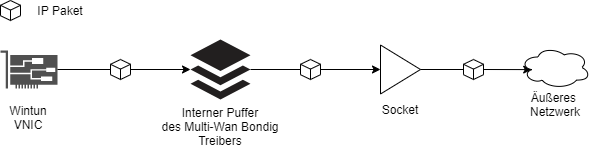
\includegraphics[width=1\textwidth]{Verarbeiten_von_IP_Paketen_in_einem_Thread.png}
    \caption[Verarbeitung von IP Paketen in einem Thread]{Verarbeitung von IP Paketen in einem Thread} 
\end{figure}
\ \\